% BREDEX LaTeX Template
%  \documentclass is either ``bxreport'' or ``bxarticle''
%% %                 option is bxpaper
%% \documentclass{bxarticle}
%% % ----------------------------------------------------------------------
%% \begin{document}
%% \title{}
%% \author{}
%% % \author*{Hauptautor}{Liste der Nebenautoren}
%% \maketitle
%% % ----------------------------------------------------------------------
%% \bxversion{0.1}
%% %\bxdocinfo{STATUS}{freigegeben durch}{freigegeben am}{Verteilerliste}
%% \bxdocinfo{DRAFT}{}{}{}
%% % ----------------------------------------------------------------------

%% \end{document}


\index{Languages!AUT}
\index{AUT!Languages}
\index{Edit!AUT Properties}
\index{AUT Properties!Edit}
\index{AUT Properties!AUT ID}
\index{AUT ID!AUT Properties}
\index{AUT!New}
\index{New!AUT}
\index{AUT!Define}
\index{Define!AUT}
\index{AUT ID}

Once you have created a \gdproject{}, you can define (and edit) \gdauts{}. 
You can define a new \gdaut{} straight after creating the \gdproject{} in the \gdproject{} wizard or you can do it later on via the \gdproject{} properties \bxpref{projectproperties}. 

\bxtipp{If you will be starting your \gdaut{} with the \bxname{gdrun} command \bxpref{gdrun}, then you can automatically define your \gdaut{} \bxpref{createAUTDef}}

The \gdaut{} dialog (\bxfigref{autdialog}) appears when you define or edit an \gdaut{}. 

\begin{figure}[h]
\begin{center}
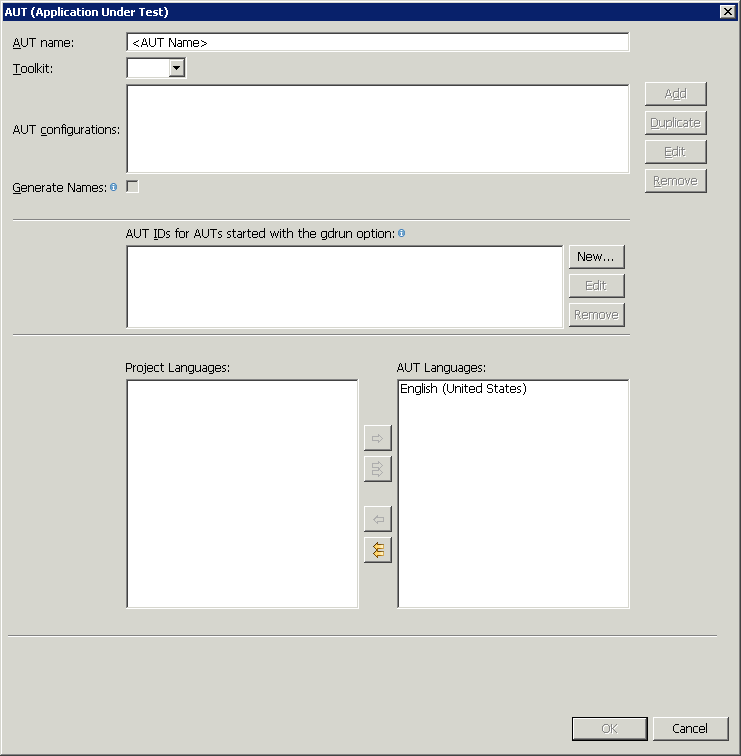
\includegraphics[width=12.5cm]{Tasks/AUTs/PS/autdialog}
\caption{AUT Dialog}
\label{autdialog}
\end{center}
\end{figure}


\begin{enumerate}
\item Enter a meaningful and unique \gdaut{} name. This is used to easily identify the \gdaut{} later. 
\item Select the toolkit the \gdaut{} uses from the combo box. 
\item If you choose RCP, decide whether or not \gd{} should generate names for components in the \gdaut{} which have not been named by your developers \bxpref{RCPgenerate}. We recommend leaving this option checked, as it increases the robustness of your tests. 
\item If you will be starting this \gdaut{} using the \bxname{gdrun} command \bxpref{gdrun}, or if the \gdaut{} will be launched from another \gdaut{} during the test \bxpref{TasksLenientTest}, then enter the ID(s) for these \gdauts{} here. 
\textbf{IDs for \gdauts{} started by the \bxname{gdrun} command}\\
You can choose the \gdaut{} IDs for \gdauts{} started by the \bxname{gdrun} command, as you will enter the \gdaut{} ID as a parameter when you start the \gdaut{} \bxpref{gdrun}.

\textbf{IDs for \gdauts{} launched by other \gdauts{}}\\
The \gdaut{} ID will take a specific form \bxpref{TasksLenientTest} and must be defined as such in the \gdaut{} definition.
 
\bxtipp{If you will be starting your \gdaut{} from \gd{}, via an \gdaut{} configuration \bxpref{configuringaut} then you do not need to enter any IDs here.}
\item From the list of \gdproject{} languages, select which languages are supported by the \gdaut{}. 

The languages you select are the languages the \gdaut{} can be started in.  You will be able to translate the data in your \gdcases{} into these languages so that a \gdsuite{} will test the \gdaut{} in the right language. 

\bxwarn{If you are editing the \gdaut{} and remove an  \gdaut{} language for which you have already specified data, this will result in the data for that language being lost. }

\item If you want to start this \gdaut{} via \gd{}, you can now click \bxcaption{Next} to create an \gdaut{} configuration for this \gdaut{} \bxpref{configuringaut}.
\end{enumerate}

If you want to  configure the \gdaut{} later, you can click \bxcaption{Finish} to create the \gdproject{} as it is. You can configure the \gdaut{} later via the \gdproject{} properties \bxpref{projectproperties}. 

If you do not require an \gdaut{} configuration, because you will be starting the \gdaut{} using the \bxname{gdrun} command \bxpref{gdrun}, then you do not need to create an \gdaut{} configuration. 

\clearpage
